\documentclass[a4paper]{article}

\usepackage[portuguese]{babel} \usepackage[utf8]{inputenc}
%\usepackage{indentfirst}
\usepackage{graphicx}
\usepackage{verbatim}
\usepackage[T1]{fontenc}
\usepackage{wrapfig}
\usepackage[tmargin=1.2in,bmargin=1in]{geometry}

\begin{document}

\setlength{\textwidth}{16cm} \setlength{\textheight}{22cm}

\title{\Huge\textbf{Protocolo de Ligação de
    Dados}\linebreak\linebreak\linebreak\linebreak \Large\textbf{Relatório \\
    Trabalho1}\linebreak\linebreak\linebreak
\includegraphics[height=6cm,
    width=7cm]{feup.pdf}\linebreak \linebreak \Large{Mestrado Integrado em
    Engenharia Informática e Computação} \linebreak \linebreak \Large\textbf{Redes de
Computadores}\linebreak}

\author{Hugo Ari Rodrigues Drumond --- 201102900 --- hugo.drumond@fe.up.pt \\
    José Pedro Pereira Amorim --- 201206111 --- ei12190@fe.up.pt \\ João
    Ricardo Pintas Soares --- 201200740 ---
    ei12039@fe.up.pt\linebreak\linebreak\linebreak \\ \\ Faculdade de
    Engenharia da Universidade do Porto \\ Rua Roberto Frias, 4200--65 Porto,
    Portugal \linebreak\linebreak\linebreak \linebreak\linebreak\vspace{1cm}}
    \maketitle \thispagestyle{empty}

\newpage

\section{Introdução}
%indicação dos objectivos do trabalho e do relatório; descrição da lógica do
%relatório com indicações sobre o tipo de informação que poderá ser encontrada
%em cada uma secções seguintes
Este trabalho laboratorial, desenvolvido no âmbito da Unidade Curricular de
Redes de Computadores (RCOM), teve como objetivo implementar um protocolo de
ligação de dados, do tipo acknowledged connection-oriented, e testá-lo em
diversas situações de stress de modo a verificar a sua robustez. Ao longo deste
relatório, serão descritos os aspetos fundamentais do referido trabalho,
permitindo obter um conhecimento detalhado deste. Será apresentada a
arquitetura, estrutura do código, casos de uso principais, protocolo de ligação
lógica e de aplicação. No mesmo sentido, serão apresentadas a validação dos
resultados e os elementos de valorização.

\section{Arquitectura}
%blocos funcionais e interfaces
O nosso software foi desenvolvido de maneira a tirar o máximo proveito da
estratégia de encapsulamento. O que permite: modificar, fazer novas
implementações, alterar técnicas de integridade de dados, etc, sem que haja
incompatibilidades ou quebra das interfaces de cada camada. Embora esta ideia
de isolamento tenha surgido nas linguagens de programação orientadas a objetos,
o código em C permite seguir este ideal pelo uso da palavra static. Tal, faz
com que um elemento só seja visível no ficheiro onde está declarado e definido.
A técnica usada pelo nosso código foi declarar a API (funções e estruturas de
retorna de informação public) de cada camada (classe) nos headers. E, nos
respetivos ficheiros de código fazer a definição da API\@; e a declaração e
definição das funções e estruturas auxiliares e de controlo com a palavra
static (private).
\\\newline\textbf{Resultando no seguinte esboço arquitectural:}\\\newline
\centerline{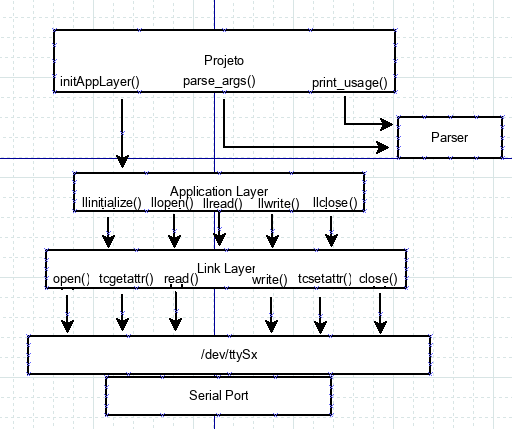
\includegraphics{API.png}}

\section{Estrutura do código}
%APIs, principais estruturas de dados, principais funções e sua relação com a
%arquitetura

\subsection{Organização dos ficheiros e código}
\centerline{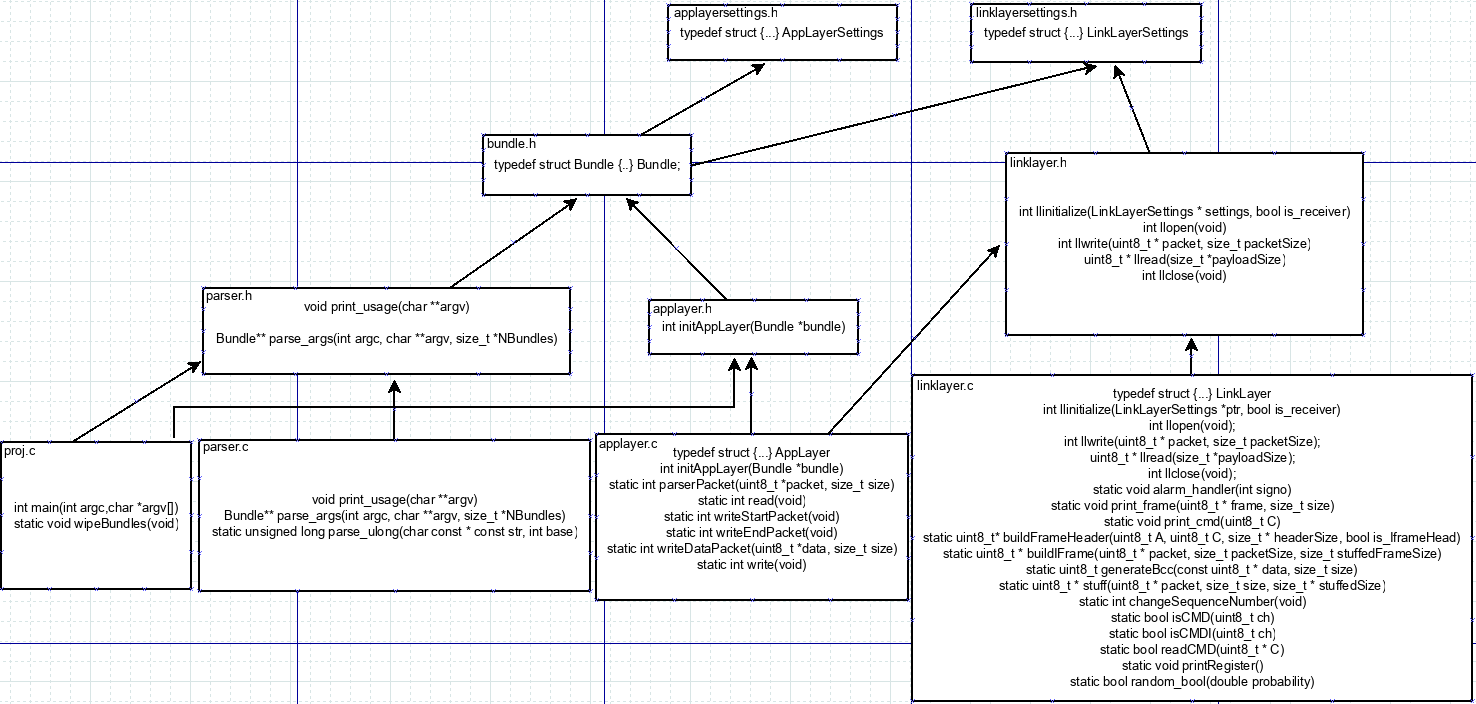
\includegraphics[scale=0.70]{organizacaoFicheirosECodigo.png}}

\subsection{Estruturas}
\begin{figure}[h]
    \centering
    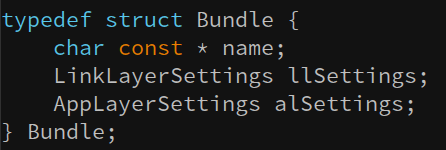
\includegraphics[width=0.45\textwidth]{bundleStruct.png}
    \caption{Estrutura Bundle presente no ficheiro \textit{bundle.h}}
\end{figure}
No \textit{bundle.h} encontra-se uma estrutura chamada Bundle cujo objetivo é
guardar os settings que recebemos da linha de comandos. O name é um nome a que
queremos chamar ao Bundle, e as estruturas constituintes do Bundle são para os
settings de cada camada. O LinkLayerSettings está declarado no ficheiro
\textit{linklayersettings.h} e contém os seguintes argumentos: port, timeout,
numAttempts, payloadSize e baudrate.
\begin{figure}[h]
\centering
    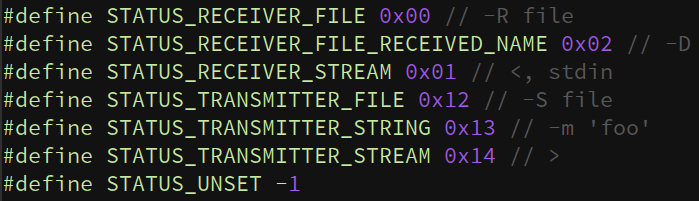
\includegraphics[width=0.45\textwidth]{status.png}
    \caption{Defines modo de operação e tipo IO no ficheiro
    applayersettings.h}
\end{figure}\\
O AppLayerSettings está declarado no
ficheiro \textit{applayersettings.h} e contém os seguintes argumentos: status,
packetBodySize, filename e um union Io que pode ser um apontador para um
ficheiro, para uma string ou nulo. Para além disso, encontram-se lá defines que
o parser usa para indicar como aceder ao Union Io e qual o modo de
operação.\\\newline

As estruturas mais importantes do nosso programa são: Applayer e LinkLayer.
Estão presentes, respetivamente, nos ficheiros: \textit{applayer.c} e
\textit{linklayer.c}.\\
\begin{figure}[h]
\centering
    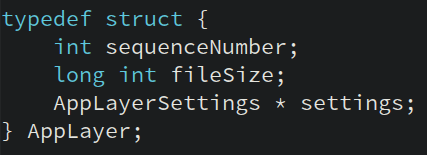
\includegraphics[width=0.45\textwidth]{applayerStruct.png}
    \caption{Estrutura AppLayer presente no ficheiro applayer.c}
\end{figure} \\
Na estrutura Applayer: usamos sequenceNumber para que
possamos identificar se houve algum pacote de dados perdido, e se tal acontecer
recuperar desse erro; fileSize é preenchido com o tamanho do ficheiro a
transmitir ou vai sendo atualizado consoante recebemos informação, para
depois compararmos com o pacote de controlo que vem no fim; e, settings que
aponta para um estrutura AppLayerSettings que foi preenchida pelo parser.\\
\begin{figure}[h]
\centering
    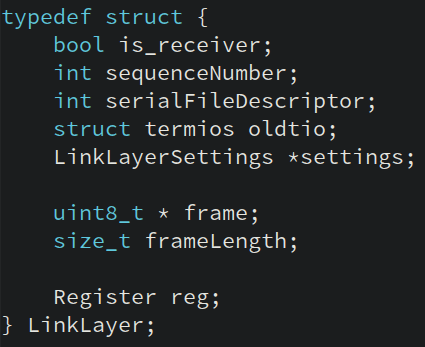
\includegraphics[width=0.45\textwidth]{linklayerStruct.png}
    \caption{Estrutura LinkLayer presente no ficheiro linklayer.c}
\end{figure}
\\ No
caso de LinkLayer: is\_receiver indica o modo de operação; sequenceNumber, a
trama de informação esperada ou a enviar; serialFileDescriptor, o descritor da
porta série aberta; oldtio, informação da porta série a ser reposta no fim da
conexão; settings, apontador para uma estrutura do tipo LinkLayerSettings onde
se encontram as configurações passadas pela linha de comandos que só interessam
a esta camada; frame, apontador para uma trama de informação unstuffed criada
na função \textit{llinitialize} com o tamanho máximo esperado; frameLength, tamanho da
trama de informação recebida; finalmente, temos uma estrutura chamada Register
que guarda ocorrências.

%\begin{wrapfigure}{R}{0.45\textwidth}
%\centering
    %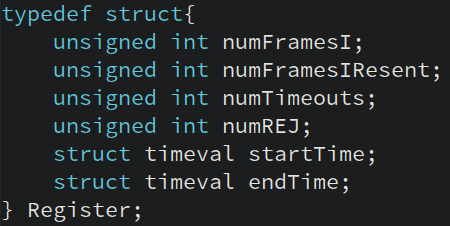
\includegraphics[width=0.45\textwidth]{registerStruct.png}
    %\caption{Estrutura de registo de ocorrências presente no ficheiro
    %linklayer.c}
%\end{wrapfigure}

\subsection{Funções}
\subsubsection{linklayer}
\textbf{\textit{static bool readCMD(uint8\_t * C);}}\\
Esta é a função mais importante do nosso código, e tem o objetivo de reconhecer
qualquer comando válido, seja ele uma trama de dados ou de controlo. É
retornado true se for encontrada uma sequência de bytes válida, isto é, uma
trama bem formada em todos os sentidos; *C, sendo C o endereço de um variável
criada por quem chamou a função. É preenchido com o tipo de comando
quando estamos no estado apropriado,
por exemplo: C\_DISC, C\_UA, C\_I\_N, C\_RR, etc.
Progredi-se na máquina de estados quando há um byte bom. Ou retrocede-se
quando há algum byte não esperado. O destuffing, tal como a verificação da integridade dos
dados é feita nesta função. Há uma divergência na máquina de estados que é
consequência de haver dois tipos de tramas. Quando estamos nesse estado e
recebemos um F, e sendo *C um comando da trama de controlo é retornado true,
que simboliza que foi recebido uma sequência válido no tempo configurado para o
alarm. De forma semelhante, é feita a verificação para o caso da trama de
informação. Se estivermos no estado divergente e se *C for um comando válido
para essa trama e o byte recebido for diferente de F dá-se início ao processo
de preenchimento do membro frame da estrutura linkLayer. Sem stuffing mas com
todos os bytes constituintes da trama. É também nesta parte do código onde se
pode gerar erros de teste nas tramas com um dada probabilidade. A estratégia
tomada foi alterar o BBC1(Header) ou o BBC2(Body) no caso da função de
probabilidade \textit{random\_bool(double probabilidade)} tiver retornado true.
As tramas de Informação com o cabeçalho bom mas com BBC errado no campo de
dados são tratadas de forma especial. É também retornado true, no entanto o
llread terá de verificar se o último byte da trama lida (linkLayer.frame) é
F ou não. Porque o F só é adicionado se a trama não tiver erros. Cabe ao
\textit{llopen}, \textit{llread}, \textit{llwrite} e ao \textit{llclose} decidir o que fazer, consoante
o tipo de comandos que recebem, *C, sempre analisando o retorno.\linebreak

\noindent\textbf{\textit{int llinitialize(LinkLayerSettings *ptr, bool
is\_receiver);}}\\
Esta função, tem de ser corrida antes de qualquer outra, e tem o objetivo de: preencher os dados iniciais da estrutura
linkLayer; instalar o signal handler; e, alocar memória para
linkLayer.frame. De início usámos a função signal (que
está deprecada), mas acabámos por mudar para função sigaction porque após um sinal alarm
o handler levava reset. Resultado num crash do programa. Todos os argumentos
são usados para inicializar valores na estrutura linkLayer.\linebreak

\noindent\textbf{\textit{int llopen(void);}}\\
Abre a porta série e configura-a com os settings necessários passados pela linha de
comandos, presentes em linkLayer.settings->{opção}. E guarda as configurações
antigas para posterior restauração. Na parte final do código temos um conjunto
de ifs dentro do while de tentativas em que se trata do processo inicial de
estabelecimento da conexão, que depende do modo de operação. Aproveita a função \textit{readCMD} para assim
evitar criar outra máquina de estados só para este caso específico. Optámos por
tratar do caso especial da trama de controlo UA poder ser
perdida ou haver timeout do emissor no \textit{llread}, uma vez
que poderíamos desperdiçar algum tempo nesta função à espera de alguma trama.
\linebreak

\noindent\textbf{\textit{uint8\_t* llread(size\_t *payloadSize);}}\\
Trata de retornar a payload com um determinado tamanho indicado por
*payloadSize à applayer. A estrutura da função é semelhante à do
\textit{llwrite}, no entanto é bem mais
extensa. Um conjunto de ifs fechados por um while de tentativas. No entanto,
temos um if bloqueante que separa a falha no estabelecimento da conexão das
restantes situações. Que é devido à possibilidade do emissor enviar uma trama de controlo SET,
novamente. Uma vez analisada essa parte, temos ifs para verificar se: número de
sequência esperado mas houver corrupção da parte dos dados; número de
sequência não esperado e corrupção da parte dos dados; trama de informação
perfeita; trama duplicada; disconnect; trama válida mas não esperada(else). O
tratamento dos casos ficou bastante facilitado uma vez que a função
\textit{readCMD} é um máquina de estados completa, que retorna por
argumento(apontador) o tipo de trama quando existe uma sequência válida de
bytes esperados(tramas independentemente do tipo, desde que sejam válidas). \linebreak

\noindent\textbf{\textit{int llwrite(uint8\_t *packet, size\_t packetSize);}}\\
Envia uma trama de dados com um determinado tamanho e espera pelo retorno para
saber se o receptor recebeu com sucesso a mensagem. Segue o mesmo
princípio do \textit{llread}, um conjunto de ifs dentro de um while de
tentativas. Cada um dos ifs analisa um determinado caso: recebeu um RR errado;
RR certo; REJ certo; REJ errado; DISC; e, comando não esperado(else).\linebreak

\noindent\textbf{\textit{int llclose(void);}}\\
Nesta função tratamos de terminar a conexão. Lá podemos encontrar uma estrutura
semelhante à parte final da função \textit{llopen}. O registo de ocorrências é
impresso, variáveis alocadas dinamicamente são limpas, configurações da porta
série antiga são restauradas, a porta é fechada, etc.\linebreak

\noindent\textbf{static uint8\_t* buildFrameHeader(uint8\_t A, uint8\_t C,
size\_t * headerSize, bool is\_IframeHead);}\\
Esta função trata de retornar a cabeça de uma trama,
is\_IframeHead, com uma dada configuração. O tamanho da trama é retornado por
argumento. A trama devolvida por esta função está pronta para ser enviada no caso de
ser uma trama de controlo, ou para juntar no caso da de informação. O
stuffing e o cálculo do bcc são aqui feitos.\linebreak

\noindent\textbf{\textit{static uint8\_t * stuff(uint8\_t * packet, size\_t size,
size\_t * stuffedSize);}}\\
Recebe um pacote com um dado tamanho, e devolve o packet stuffed com o BCC
acoplado e o respetivo tamanho por argumento. Esta função só é chamada pelo
\textit{buildIframe}.
\linebreak

\noindent\textbf{\textit{static uint8\_t * buildIFrame(uint8\_t * packet, size\_t
packetSize, size\_t * stuffedFrameSize);}}\\
Constrói uma trama de informação. Recebe o packet e o tamanho. E devolve a
trama de informação pronta a enviar e o tamanho por argumento. A trama é
construída por partes: é feita a cabeça; depois é feito o BCC e o stuffing do
pacote que é realizado pela função \textit{stuff}; e depois junta-se as
duas partes e adiciona-se um F.\linebreak

\noindent\textbf{\textit{static bool isCMD(uint8\_t ch);}}\\
Verifica se o byte ch é um campo de controlo válido de uma trama de controlo. \linebreak

\noindent\textbf{\textit{static bool isCMDI(uint8\_t ch);}}\\
Verifica se o byte ch é um campo de controlo válido de uma trama de informação. \linebreak

\noindent\textbf{\textit{static bool random\_bool(double probability);}}\\
Função que devolve true com uma dada probabilidade.

\subsubsection{applayer}
\noindent\textbf{\textit{int initAppLayer(Bundle *bundle);}}\\

%\linebreak
\noindent\textbf{\textit{static int read(void);}}\\

%\linebreak
\noindent\textbf{\textit{static int write(void);}}\\

\subsubsection{parser}

\noindent\textbf{\textit{Bundle** parse\_args(int argc, char **argv, size\_t *NBundles)}}\\

\section{Casos de uso}
%identificação; sequências de chamada de funções
O utilizador só pode interagir com a nossa aplicação através da linha de
comandos. Criámos um caso de usos bastante completo, que permite ao utilizador
mudar todas as opções do linkLayer e da applicacationLayer, que têm impacto na
transferência de dados. Para além disso, o parser aceita um número ilimitado de
portas séries quer sejam destinadas a receber ou enviar, e as respetivas
configurações. Cada uma separada com o símbolo +. Para ver quais as opções que
a nossa aplicação suporta basta corrê-la com a opção -h, serius -h. Também
incluímos alguns exemplos de uso. Lá podemos encontrar o nome Bundle que
basicamente significa um conjunto de opções (Options:) para uma dada porta
série que opera de uma dada maneira (Mode:), receptor ou emissor. Por
exemplo:\\\newline serius -d'/dev/tty100' -b115200 -t4 -r10 -f150 -s90
-S'pinguim.gif' + -d'/dev/tty200' -S'pinguim.gif'\\\newline Neste exemplo, os
seguintes settings são aplicados na porta série tty100: baudrate, timeout,
retries, tamanho máximo do payload (unstuffed) e o tamanho máximo da parte dos
dados do pacote de informação. E na tty200 os defaults são usados para todas
essas opções e para as restantes. Em ambos os casos as portas série atuam como
emissoras e enviam o ficheiro pinguim.gif para possivelmente computadores
diferentes. Um dos computadores receptores teria um processo serius iniciado
com os seguintes argumentos:\\\newline serius -d '/dev/tty300' -b 115200 -D\\
Cria um ficheiro com o nome que vem no pacote de controlo start, e coloca lá a
informação que recebe. \\\newline E o outro:\\\newline serius -d '/dev/tty400'
-R 'received.gif' \\\newline De início, tínhamos em mente correr cada Bundle
numa thread. Possibilitando transferir/receber de várias fontes simultâneamente
via porta série, no entanto, não houve tempo para o fazer. O mesmo sucedeu com
as pipes e a redireção da shell, cuja ideia era respetivamente: enviar
informação acabada de ser processada; e, método alternativo de guardar
ficheiros ou de os receber.\\Entre a opção e o argumento tanto faz haver ou nao
haver espaços, -b115200 = -b 115200.
\\\newline\textbf{Diagrama de casos de uso:}\\\newline
\centerline{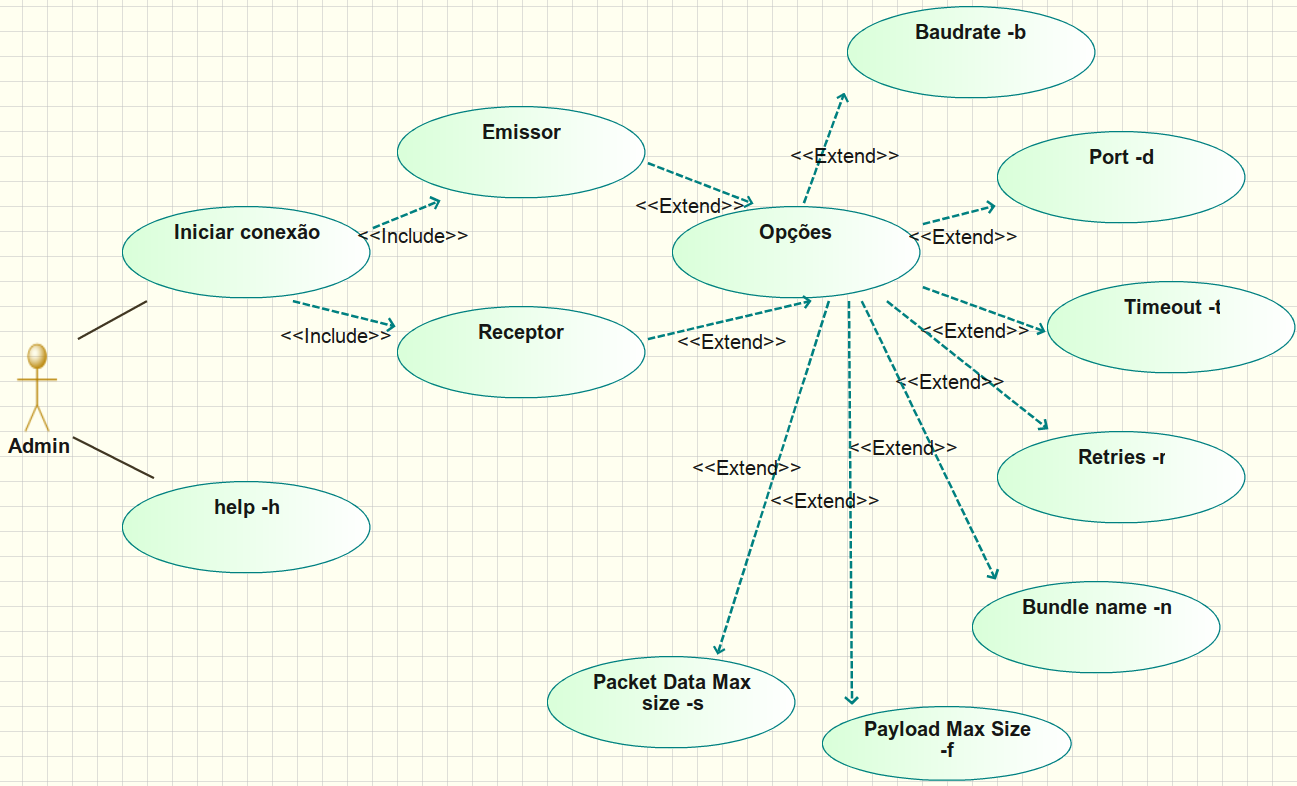
\includegraphics[scale=0.6]{useCases.png}}

\section{Protocolo de ligação lógica}
%identificação dos principais aspectos funcionais; descrição da estratégia de
%implementação destes aspectos com apresentação de extratos de código
Falar sobre a máquina de estados; poupança de ciclos for, destuffing e bbc; mostrar o código da máquina de
estados, llwrite, llread. Ligação entre funções do linklayer

\section{Protocolo de aplicação}
%identificação dos principais aspectos funcionais; descrição da estratégia de
%implementação destes aspectos com apresentação de extractos de código
Falar sobre ter uma só função public; pacote start, pacote end; ligação entre
funções da applayer

\section{Validação}
%descrição dos testes efectuados com apresentação quantificada dos resultados,
%se possível
falar sobre os printfs; tentativa de fazer debugging com break points;
vericacao da implementacao atraves de portas serie virtuais, socat; e nos pcs
da feup

\section{Elementos de valorização}
%identificação dos elementos de valorização implementados; descrição da
%estratégia de implementação com apresentação de pequenos extratos de código
Fizemos todos falar e mostrar cada um deles

\section{Conclusões}
%síntese da informação apresentada nas secções anteriores; reflexão sobre os
%objectivos de aprendizagem alcançados

\end{document}
